Durante un desastre natural se puede ver afectada la infraestructura de
comunicaciones como Internet o redes móviles haciendo difícil para las personas
recolectar y diseminar información. Ante este problema es que se han presentado
soluciones basadas en redes DTN para poder comunicar a las personas en estas
situaciones. En este tipo de redes, al utilizar copias de mensajes para tratar
de llegar al destino, puede presentar problemas de consumo de energía causado
por la transmisión de mensajes entre los nodos que influye en el tiempo en que
una red puede mantenerse activa. Debido a que en un escenario de desastre el
acceso a energía para recargar los dispositivos puede ser escasa, es que se debe
tener cuidado con el consumo de energía de los protocolos.


Como primer acercamiento a la solución final de esta tesis se ha presentado un
protocolo llamado \textit{MetaRouter}, que es estático y permite asignar
manualmente el protocolo a ejecutar por un nodo permitiendo crear redes híbridas
que pueden reducir el consumo de energía relacionado con la transmisión de
mensajes que se puede medir directamente con el \overhead{} de mensajes. Este
protocolo fue publicado en la \textit{2nd International Conference on Information
and Communication Technologies for Disaster Management}
\cite{paper_evaluacion_nosotros}. Además, \textit{MetaRouter} fue presentado en
forma de \textit{poster} en la \textit{Spring School of Networks} en las
Jornadas Chilenas de la Computación 2015 y le fue otorgado el premio IETF
\textit{Internet Engineering Task Force} como mejor trabajo relacionado con DTN.


Algunos protocolos como \epidemic{} \cite{amin_vahdat_epidemic_2000} y
\maxprop{} \cite{burgess_maxprop:_2006} tienen buenas tasas de entrega pero
presentan a su vez un alto \overhead{} de mensajes, mientras que otros como
\syw{} \cite{spyropoulos_spray_2005} y \syf{} \cite{spyropoulos_spray_2007}
presentan un bajo \overhead{} pero al mismo tiempo una baja tasa de entrega.
Esta información permite pensar que entonces existe la oportunidad de mejorar el
desempeño de la red si es que se aplica un protocolo distinto dependiendo del
objetivo que se quiera optimizar. En el caso de una red orientada a desastres
interesa minimizar el consumo de energía sin perjudicar tanto la tasa de entrega
ni la latencia. Además, debido a modelos como PDM
\cite{uddin_post-disaster_2009} donde existen roles en los nodos de la red con
distintas movilidades, es que se explora la posibilidad de asignar un protocolo
distinto dependiendo del tipo de movimiento que la persona o vehículo que tiene
el dispositivo móvil realice.

A continuación se presenta el desarrollo del protocolo \textit{MetaRouter}, el
cual permite a los nodos utilizar distintos protocolos DTN del estado del arte
de acuerdo a: su característica de movilidad y densidad de vecinos y las
característica de los nodos que encuentra en su camino. Nodos con una alta
movilidad pueden explorar el área afectada y transportar los mensajes más lejos
mientras que los nodos con una movilidad menor tienen mayor probabilidad de
encontrar al destino en sus cercanías.

En una primera etapa exploratoria se ejecutaron los protocolos bajo el modelo de
movilidad PDM y con configuraciones estándar. Esta información permite averiguar
el comportamiento de los protocolos bajo las métricas estudiadas para poder
finalmente tomar la decisión de cual asignar a que nodo de la red.


\seccion{Evaluación de protocolos DTN}

A continuación se presentan las evaluaciones de los protocolos \epidemic, \syw,
\syf, \maxprop{} y \prophet{} \cite{lindgren_probabilistic_2003} con el objetivo
de analizar como se comportan.

Las simulaciones se crearon con las siguientes configuraciones: 10 vecindarios
con 20 personas cada uno, 5 ambulancias, 5 vehículos de policía, una unidad de
reparación, 20 rescatistas, un centro de comando, 60 casas, un centro de
policía, un hospital, un centro de coordinación y un centro de rescate. Como se
mencionó anteriormente el modelo de movilidad es PDM
\cite{uddin_post-disaster_2009} debido a que permite simular una ciudad luego de
la ocurrencia de un desastre donde las personas se mueven en un vecindarios
mientras que las ambulancias y patrullas se mueven por la ciudad visitando los
centros y vecindarios entregando conectividad entre clusters de personas. Los
mensajes tienen un tamaño promedio de $500$ KB y son generados cada $120$ segundos
en algún nodo aleatorio. Cada nodo además tiene un \textit{buffer} de
almacenamiento de mensajes de $50$ MB lo cual es un valor conservador si se
considera que actualmente la mayoría de los dispositivos tienen una capacidad de
$4$ GB. Finalmente, el TTL (\textit{time-to-live}) del mensaje tiene un valor
de $360$ minutos. Cada una de las pruebas consistió en un tiempo de simulación
de $172800$ segundos o $48$ horas. Los protocolos \syw{} y \syf{} tienen un
límite de copias de $20$. Las pruebas fueron ejecutadas en \theone{}
\cite{keranen_one_2009}. Se utilizaron estás configuraciones ya que son las
utilizadas en el trabajo de Uddin et al. sobre consumo de energía en escenarios
de desastres donde se utiliza también el modelo de movilidad propuesto por
ellos \cite{uddin_intercontact_2013-1}.

\figura{Destino de los mensajes desde personas a centros.}
{\begin{tikzpicture}

  \begin{scope}[
     xshift=-7.5cm
    ,yshift=-5cm
    ,very thick
    ,node distance=1.6cm
    ,on grid
    ,>=stealth'
    ,block/.style={rectangle,draw,fill=cyan!20}
    ,comp/.style={circle,draw,fill=orange!40}
    ]

  \node [comp] (centro1) [xshift=-1cm] { Centro 1};
  \node [comp] (centro2) [right=of centro1, xshift=1cm] { Centro 2};

  \node [comp] (a) [above=of centro1, yshift=0.5cm] {A} edge [->] (centro1) edge [->] (centro2);
  \node [comp] (b) [below=of centro1, yshift=-0.5cm] {B} edge [->] (centro1) edge [->] (centro2);
  \node [comp] (c) [above=of centro2, yshift=0.5cm] {C} edge [->] (centro2) edge [->] (centro1);

  \end{scope}

\end{tikzpicture}
}{fig:envio-persona-centro}

\figura{Destino de los mensajes desde centros a centros.}
{\begin{tikzpicture}

  \begin{scope}[
     xshift=-7.5cm
    ,yshift=-5cm
    ,very thick
    ,node distance=1.6cm
    ,on grid
    ,>=stealth'
    ,block/.style={rectangle,draw,fill=cyan!20}
    ,comp/.style={circle,draw,fill=orange!40}
    ]

  \node [comp] (centro1) [xshift=-1cm] { Centro 1};
  \node [comp] (centro2) [right=of centro1, xshift=1cm] { Centro 2} edge [<->] (centro1);

  \node [comp] (a) [above=of centro1, yshift=0.5cm] {A};
  \node [comp] (b) [below=of centro1, yshift=-0.5cm] {B};
  \node [comp] (c) [above=of centro2, yshift=0.5cm] {C};

  \end{scope}

\end{tikzpicture}
}{fig:envio-centro-centro}

\figura{Destino de los mensajes entre todos los nodos.}
{\begin{tikzpicture}

  \begin{scope}[
     xshift=-7.5cm
    ,yshift=-5cm
    ,very thick
    ,node distance=1.6cm
    ,on grid
    ,>=stealth'
    ,block/.style={rectangle,draw,fill=cyan!20}
    ,comp/.style={circle,draw,fill=orange!40}
    ]

  \node [comp] (centro1) [xshift=-1cm] { Centro 1}
    edge [<->] (a)
    edge [<->] (b)
    edge [<->] (c);

  \node [comp] (centro2) [right=of centro1, xshift=1cm] { Centro 2}
    edge [<->] (centro1)
    edge [<->] (a)
    edge [<->] (b)
    edge [<->] (c);

  \node [comp] (a) [above=of centro1, yshift=0.5cm] {A}
    edge [<->, bend right=50] (b)
    edge [<->] (c);

  \node [comp] (b) [below=of centro1, yshift=-0.5cm] {B};

  \node [comp] (c) [above=of centro2, yshift=0.5cm] {C};
  
  \draw[<->] (c) .. controls +(right:3cm) and +(right:4cm) ..  (b);

  \end{scope}

\end{tikzpicture}
}{fig:envio-todos}

Para poder simular diferentes tipos de escenarios, se implementó un nuevo
sistema de generación de mensajes que permite evaluar como afectan los distintos
tipos de comunicación como mensajes desde las personas hacia los centros, entre
centros y entre todos los nodos de la red. La \ref{fig:envio-persona-centro}
ejemplifica el destino de los mensajes cuando son enviados desde los nodos $A,
B, C$ hacia los centros, en la \ref{fig:envio-centro-centro} se muestran los
destinos cuando es solo entre nodos y finalmente en la \ref{fig:envio-todos} se
muestran los destinos entre todos los nodos de la red. La idea de la
comunicación desde las personas hacia los centros es tratar de evaluar un modelo
en el cual las personas envían necesidades a las autoridades o reportan la
situación y estado de la ciudad luego de un desastre. La comunicación entre
centros trata de evaluar la situación en la cual las autoridades utilizan a la
red como soporte de las tareas administrativas. Finalmente, la comunicación entre
todos los dispositivos simula el caso en el que hay comunicación de dos vías
entre autoridades y entre personas.

Se definen los siguientes conceptos de manera tal de poder aplicarlo sobre otros
modelos de movilidad y no solamente PDM:

\begin{itemize}
  \item \textbf{Nodo explorador} tiene una alta movilidad y recorre grandes áreas
  requiriendo mayor velocidad de movimiento que otros nodos. Está asociado a los
  nodos \textit{carrier}, es decir, aquellos que comunican vecindarios o
  \textit{clusters} de nodos.
  \item \textbf{Nodo explotador} nodos con poca movilidad que aprovechan de los
  nodos exploradores para tener conectividad en la red.
\end{itemize}



Antes de realizar las pruebas, la intuición dice que protocolos con una alta
tasa de entrega son buenos candidatos a ser utilizados por los nodos
exploradores, es decir, nodos que tienen una alta movilidad deberían ejecutar
este tipo de protocolos. Por otro lado, protocolos con un bajo \overhead{} como
\syw{} y \syf{} deberían ser utilizados en nodos explotadores, es decir, con
baja movilidad debido a que se requieren menos copias para llegar a destinos que
se encuentren dentro del vecindario del nodo, asumiendo que existen en la red
nodos exploradores que pueden llevar los mensajes a lugares lejanos de la ciudad.
Para comprobar estas afirmaciones, se analizan los experimentos de la
\ref{fig:p-c}, la \ref{fig:c-c} y la \ref{fig:t-t} para identificar como se
comportan los protocolos del estado del arte en un escenario de desastre. Cada
uno de estos valores se calcula como un promedio de entre todos los nodos de la
red.


%%%%%%%%%%%%%%%%%%%%%%%%%%%%%%%%%%%%%%%%%%%%%%%%%%%%%%%%%%%%%%%%%%%%%%%%%%%%%%%%

\figuraFuente{Mensajes desde personas hacia centros, protocolos originales.}
{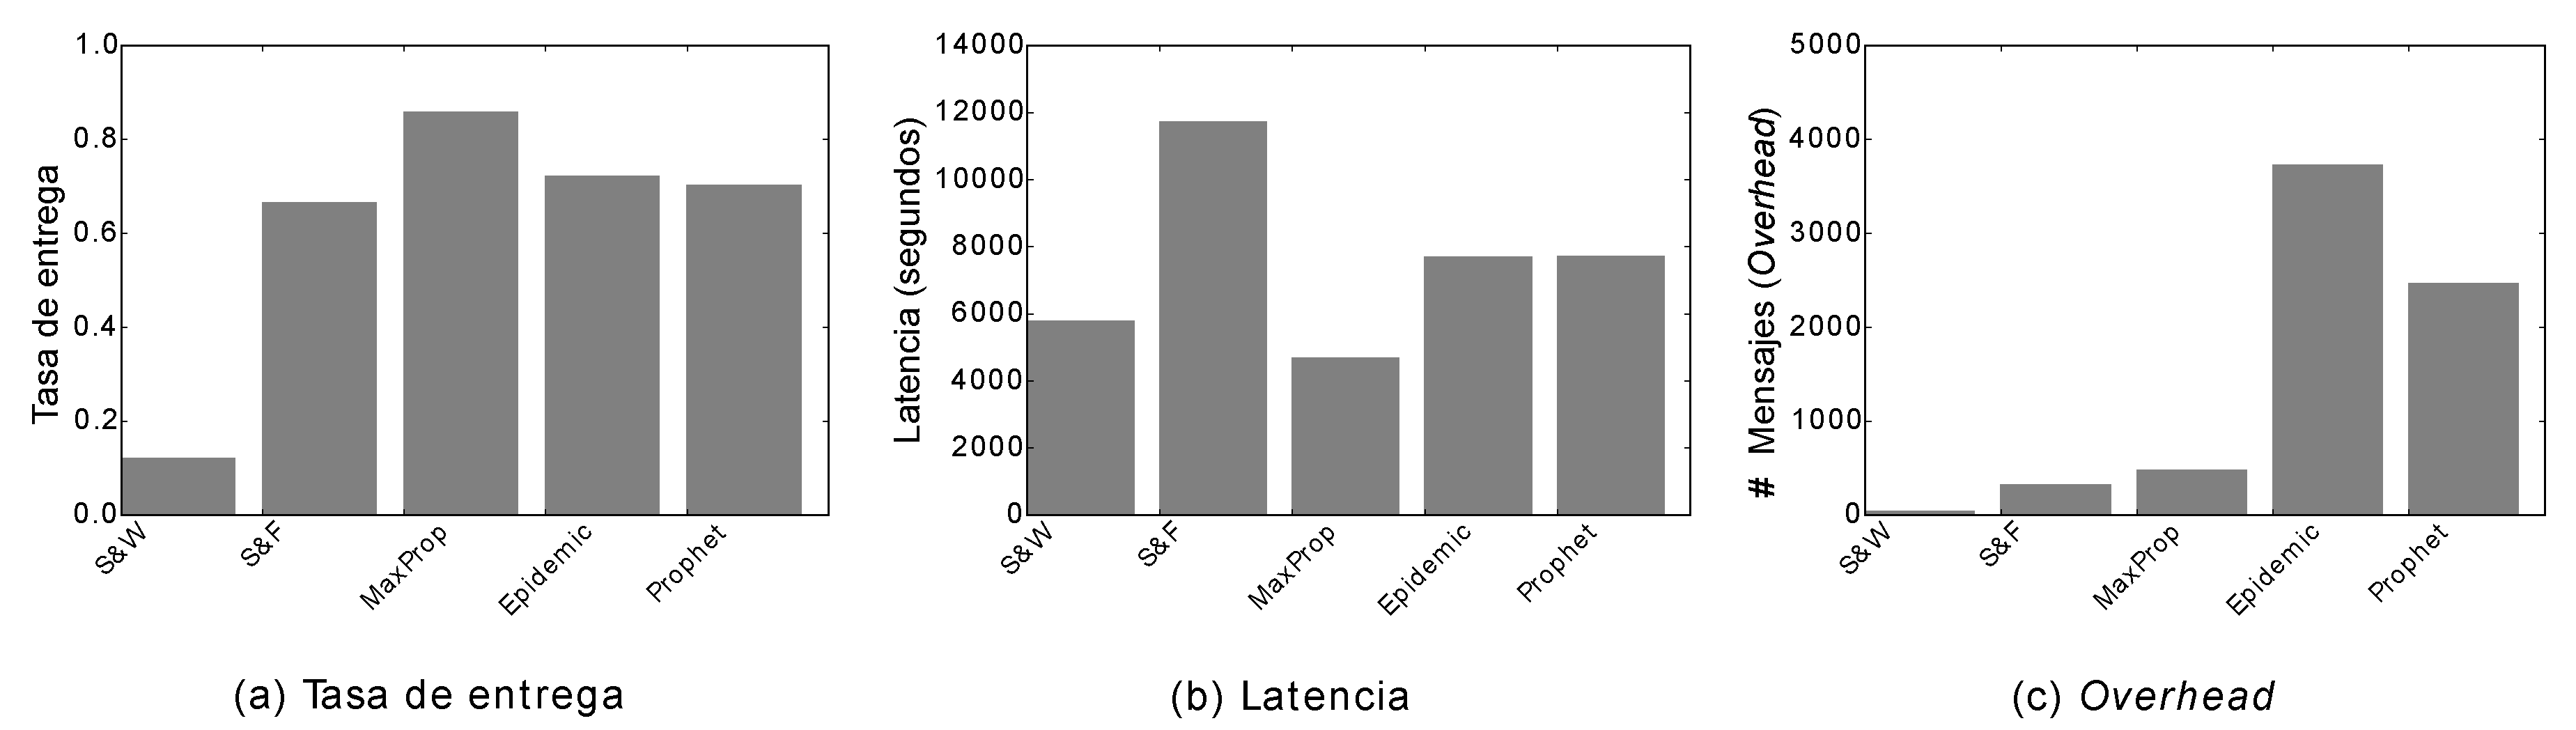
\includegraphics[scale=0.27]{desarrollo/paper_pasado/graficos/clasicos_desde_personas.eps}}{fig:p-c}
{Elaboración propia, (2015)}


\figuraFuente{Mensajes entre centros, protocolos originales.}
{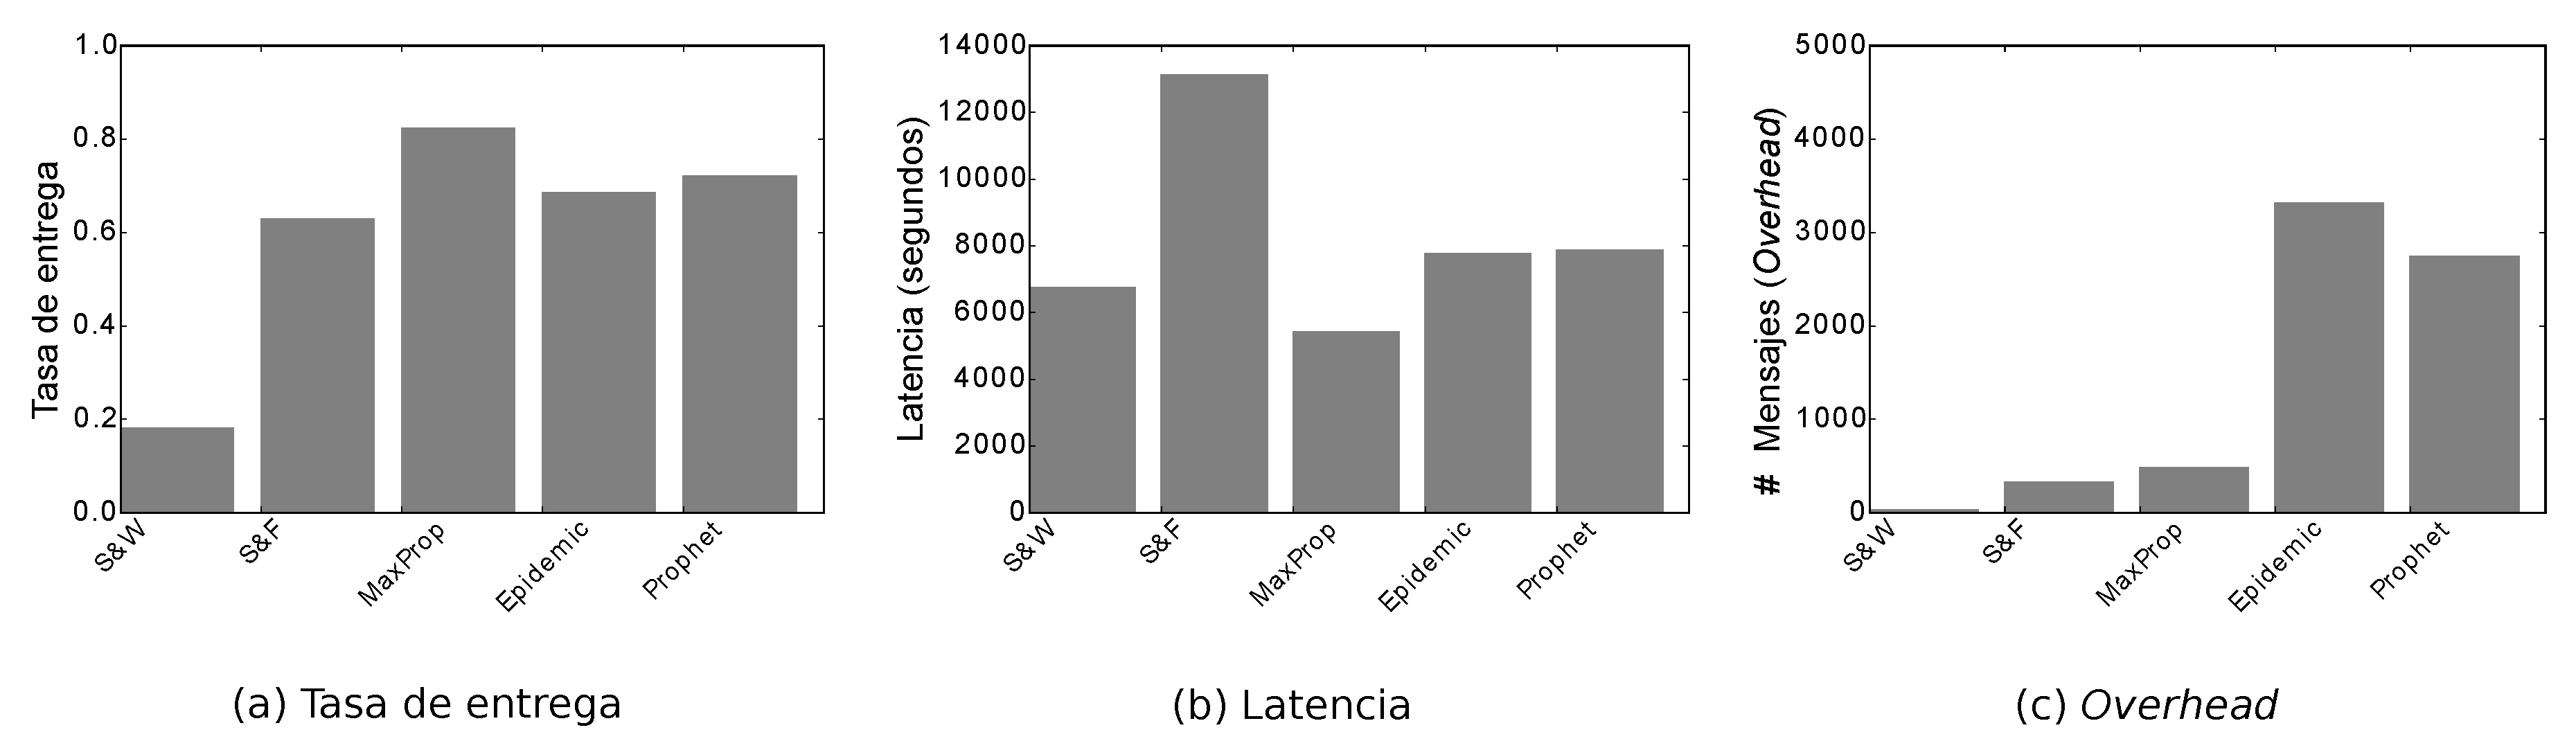
\includegraphics[scale=0.27]{desarrollo/paper_pasado/graficos/clasicos_entre_centros.eps}}{fig:c-c}
{Elaboración propia, (2015)}


\figuraFuente{Mensajes entre todos los nodos, protocolos originales.}
{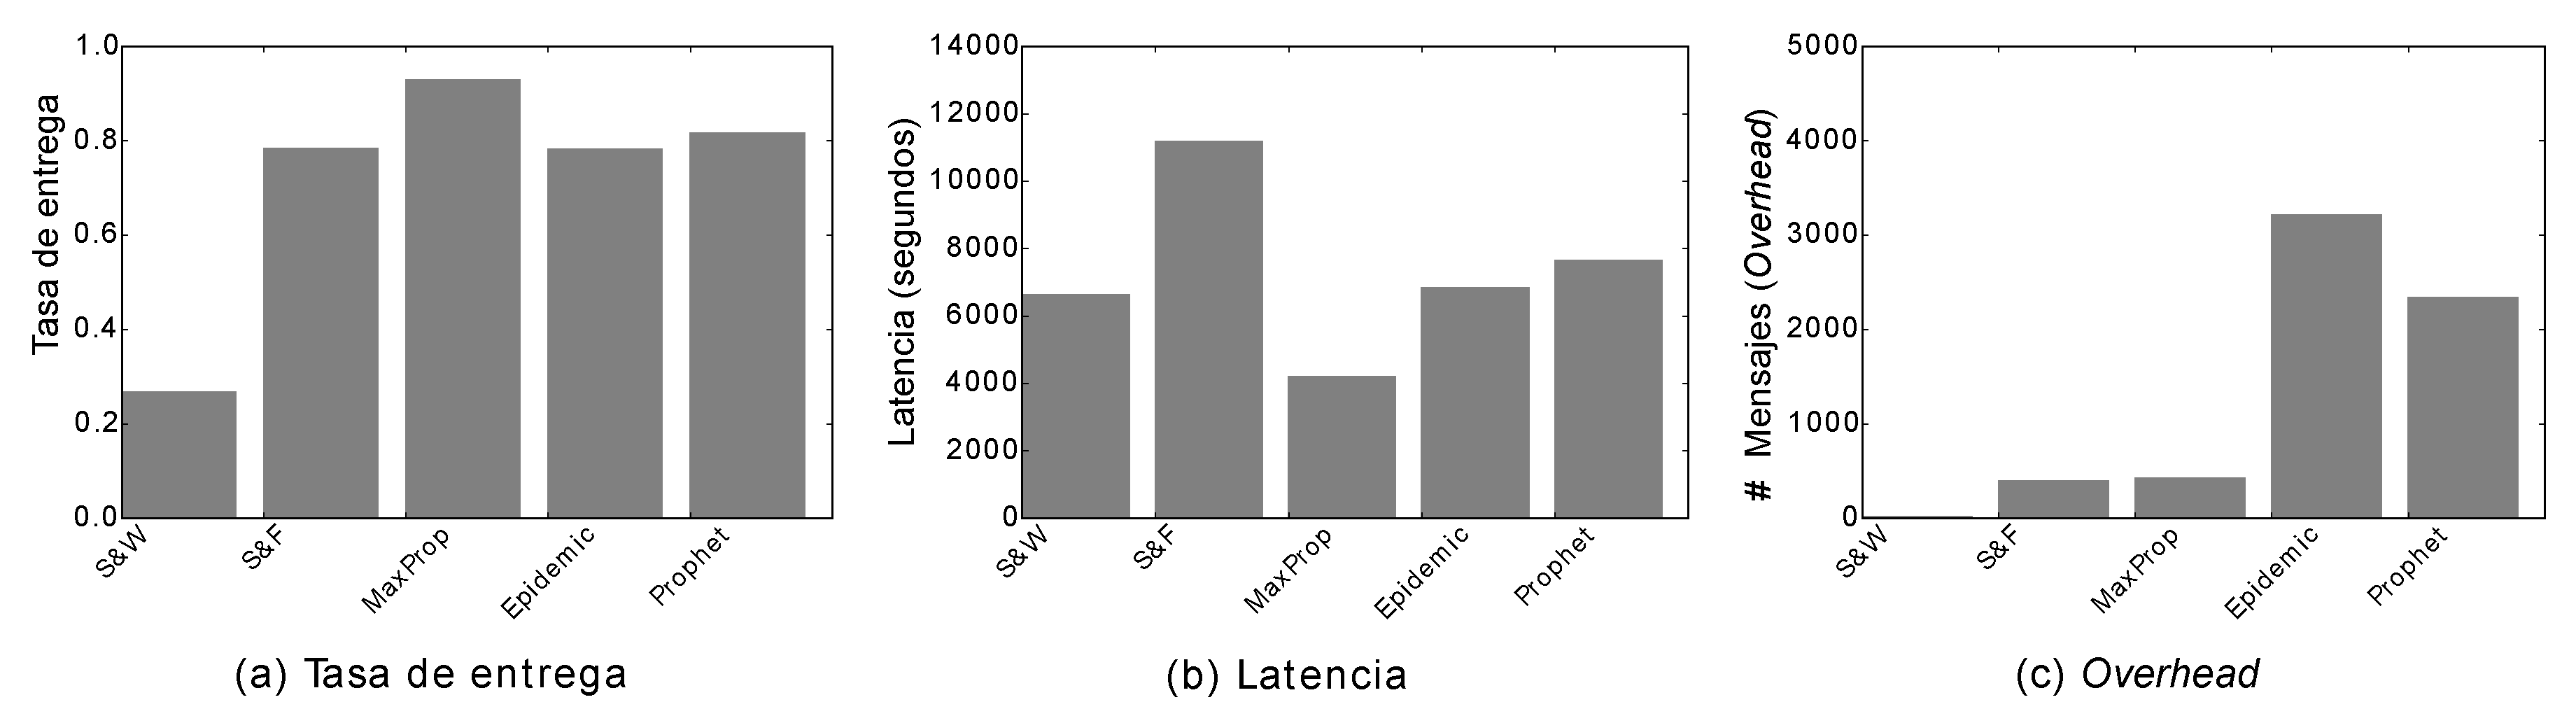
\includegraphics[scale=0.27]{desarrollo/paper_pasado/graficos/clasicos_todos.eps}}{fig:t-t}
{Elaboración propia, (2015)}

%%%%%%%%%%%%%%%%%%%%%%%%%%%%%%%%%%%%%%%%%%%%%%%%%%%%%%%%%%%%%%%%%%%%%%%%%%%%%%%%


En la \ref{fig:p-c} (a) se puede ver que el protocolo \syw{} es el que peor
desempeño tiene cuando se compara con el resto y no solamente cuando los
mensajes son desde las personas hacia los centros, si no también en los otros
casos de las \ref{fig:c-c} (a) y \ref{fig:t-t} (a), esto nos indica que la
intuición era correcta y que este sería el protocolo con menor tasa de entrega.
Cuando se miran los gráficos de \overhead{} en la \ref{fig:p-c} (c),
\ref{fig:c-c} (c) y \ref{fig:t-t} (c) se nota que este protocolo posee la
ventaja de tener el \overhead{} más bajo de los protocolos comparados, lo que se
traduce en una reducción directa de la energía consumida por el dispositivo.
Esta ventaja es causada por la inundación controlada realizada por \syw{} que
en este caso está limitada a 20 mensajes.

En el caso de \epidemic, se esperaría que tuviera una tasa de entrega mayor que
el resto de los protocolos incluso llegando hasta un nivel cercano a 1. La razón
del bajo desempeño de este protocolo es que \epidemic{} tiene un alto
\overhead{} de copias de mensajes lo que satura los \textit{buffers} obligando a
los dispositivos a descartar los mensajes más antiguos que tengan almacenados.
Esto reduce la tasa de entrega del protocolo y además le da un alto consumo de
energía relacionado con la comunicación de mensajes.

Analizando la latencia, \maxprop{} es el que es capaz de entregar los mensajes
en el menor tiempo posible debido a que la forma de calcular las probabilidades
de encuentro le permiten encontrar un mejor camino para los mensajes utilizando
Dijkstra. \syw{} también es un caso interesante de analizar debido a que tiene
un baja latencia teniendo una baja tasa de entrega. La explicación de este caso
es que \syw{} entrega pocos mensajes, pero los que entrega lo hace rápidamente
debido a que los destinos deben estar cerca para ser entregados con 20 copias.


De acuerdo a los datos obtenidos, se puede ver que el origen de los mensajes
no influencia en mayor medida el desempeño de los protocolos, al menos cuando se
comparan uno a otro. Los protocolos tienden a mantener su posición respecto a
otros si se compara respecto a cual tiene mejor tasa de entrega o peor
\overhead. La excepción es \epidemic, el cual tiene una mayor tasa de entrega
que \prophet{} cuando los mensajes son desde las personas hacia los centros que
en el resto de los casos, pero su \overhead{} aumenta si se comparan los valores
absolutos respecto a los otros gráficos (\ref{fig:c-c} y \ref{fig:t-t}).




%%%%%%%%%%%%%%%%%%%%%%%%%%%%%%%%%%%%% METAROUTER %%%%%%%%%%%%%%%%%%%%%%%%%%%%%%

\seccion{Diseño del protocolo DTN estático}

Una vez analizados los datos de cada uno de los protocolos es posible construir
\textit{MetaRouter} utilizando la información obtenida. Dado que los nodos
tienen distintos patrones de movilidad, si se le asigna un protocolo distinto a
cada uno de los tipos de nodos se puede reducir el consumo de energía.
\textit{MetaRouter} es un protocolo \textit{middleware} que actúa como una capa
de selección y va a ejecutar uno de los protocolos del estado del arte
dependiendo del tipo de nodo que lo está ejecutando. La diferencia de nodo se
hace en las dos categorías previamente presentadas: nodos explotadores (personas
en los vecindarios) y nodos exploradores (vehículos).


\figura{Diagrama de clase reducido de \textit{MetaRouter}.}
{\begin{tikzpicture}
  \begin{umlpackage}{Routing}

    \umlclass[]{MetaRouter}{
      clusterRouter : ActiveRouter \\
      carrierRouter : ActiveRouter 
    }{
      isCarrier() : boolean
    }

    \umlclass[y=-3]{ActiveRouter}{}{}

    \umlinherit[geometry=-|]{MetaRouter}{ActiveRouter}

  \end{umlpackage}
\end{tikzpicture}
}{fig:metarouter}


\textit{MetaRouter} funciona de la siguiente manera: debido a que cada nodo de
la simulación tiene un nombre único, es posible identificar a los nodos. Por
ejemplo los nodos con movilidad reducida como las personas tiene como nombre
"PERSONA\_CLUSTER" mientras que los vehículos tienen por nombre
"POLICE\_CARRIER" o "AMBULANCE\_CARRIER", luego basta con utilizar un método de
comparación de \textit{strings} como el de Java "compare" para poder identificar
si el nodo es parte de un cluster (movilidad reducida) o es un \textit{carrier}
de mensajes (alta movilidad). Esta asignación es la razón por la cual a este
protocolo se le dice ser estático, dado que depende de la asignación inicial
dada al nombre del nodo y se asume que su movilidad no cambia. La comparación de
\textit{strings} se hace en un método llamado "isCarrier" que retorna
\textit{true} si es que el nodo tiene una alta movilidad o \textit{false} si
tiene una baja. Más detalladamente, el protocolo diseñado realiza las siguientes
funcionalidades:

\begin{itemize}
  \item Un nodo decide enviarle un mensaje a otro basado en el protocolo que
    está ejecutando.
  \item Para \maxprop{} y \prophet{}, donde se utilizan los encuentros pasados
    para poder decidir si entregar o no un mensaje, todos los nodos de la red
    mantienen esa información, incluso si no ejecuta ninguno de estos
    protocolos.
  \item Si el nodo se encuentra con otro que usa el mismo protocolo para
    intercambiar los mensajes, entonces simplemente sigue las reglas normales de
    intercambio.
  \item Si el nodo decide enviar el mensaje a otro que usa otro tipo de
    protocolo, por ejemplo para enviar un mensaje desde un vecindario hacia un
    \textit{carrier}, entonces \textit{MetaRouter} convierte el mensaje al
    formato del otro protocolo.
  \item Algunos protocolos como \syw{} y \syf{} deben mantener el número de
    copias permitidos dentro de los mensajes para controlar la inundación. Hay
    dos posibilidades que \textit{MetaRouter} puede hacer: guardar el valor
    asociado al número de copias al pasar a un protocolo que no es ninguno de
    los dos anteriores o reiniciar el valor al máximo de copias disponibles.
\end{itemize}



El protocolo fue implementado en "Scala" debido a que compila a \textit{byte
code} compatible con la \textit{Java Virtual Machine} utilizada por el simulador
\textit{The ONE}, permite expresar más con menos líneas de código, permite
ocupar el paradigma funcional que evita el estado dentro de las clases y tiene
soporte para inferencia de tipado que permite reducir la verbosidad de un
programa equivalente en Java.


\figura{Diagrama de intercambio de mensajes de \textit{MetaRouter}.}
{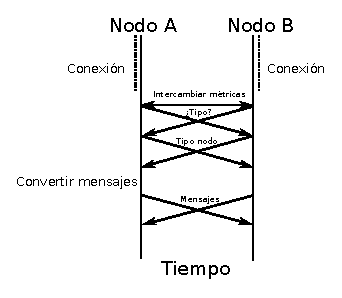
\includegraphics[scale=1.75]{imagenes/metarouter/metarouter_diagrama.eps}}{fig:metarouter-intercambio-mensajes}


El diagrama de la \ref{fig:metarouter-intercambio-mensajes} indica como funciona
la comunicación del protocolo. Hay que recordar que dado que los protocolos DTN
se implementan en la capa de aplicación, el manejo de errores es responsabilidad
de protocolos de la capa de transporte como TCP y el control de acceso a la red
por su respectiva capa. En el diagrama se puede ver que inicialmente se
intercambian las métricas de protocolos como \syf, \prophet{} y \maxprop, luego
se analiza con que tipo de nodo se va a establecer el intercambio de mensajes,
se realiza la conversión correspondiente y se le envía los mensajes que el
protocolo que está siendo ejecutado (los del estado del arte) indique que se
tienen que mandar.



\subseccion{Evaluación del protocolo estático}

Para saber si es que realmente existen mejoras respecto a los protocolos
normales, se evaluó \textit{MetaRouter} sobre el mismo escenario de los
experimentos de la sección anterior considerado las distintas fuentes de
mensajes como se ve en la \ref{fig:envio-persona-centro},
\ref{fig:envio-centro-centro} y \ref{fig:envio-todos}.


\figuraFuente{Mensajes desde personas hacia centros, \textit{MetaRouter}.}
{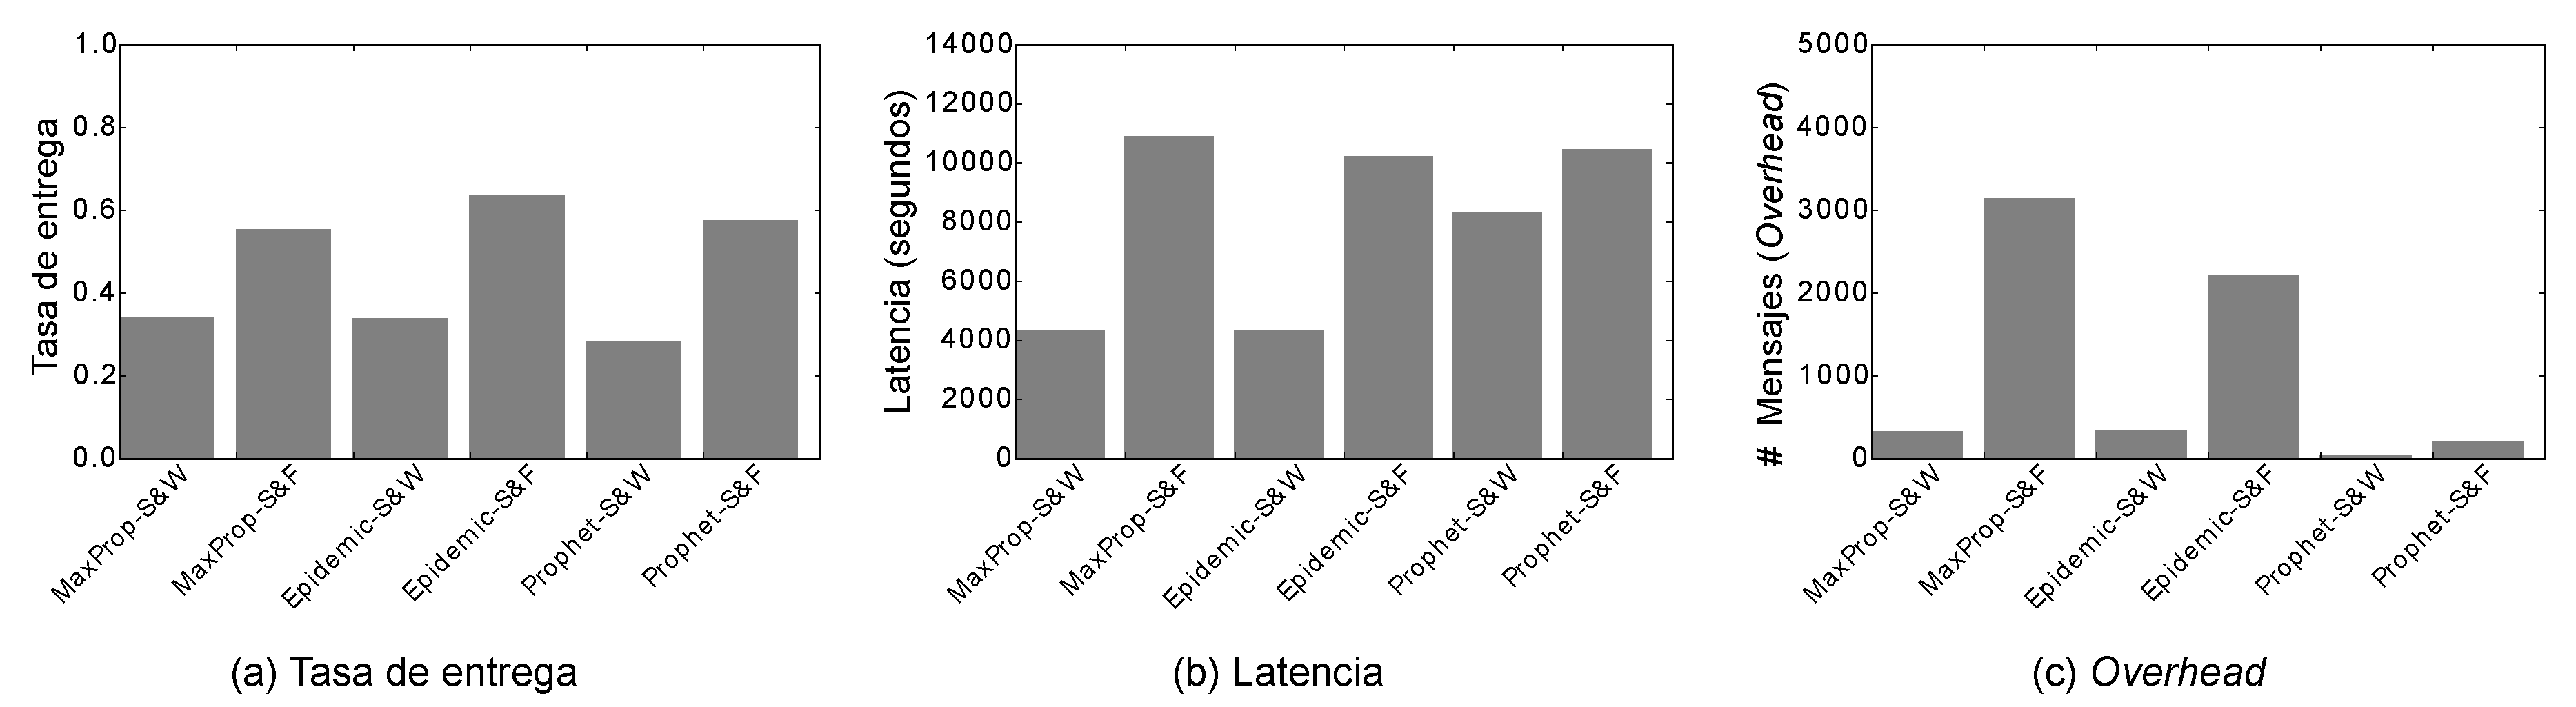
\includegraphics[scale=0.27]{desarrollo/paper_pasado/graficos/desde_personas.eps}}{fig:p-c-meta}
{Elaboración propia, (2015)}


\figuraFuente{Mensajes entre centros, \textit{MetaRouter}.}
{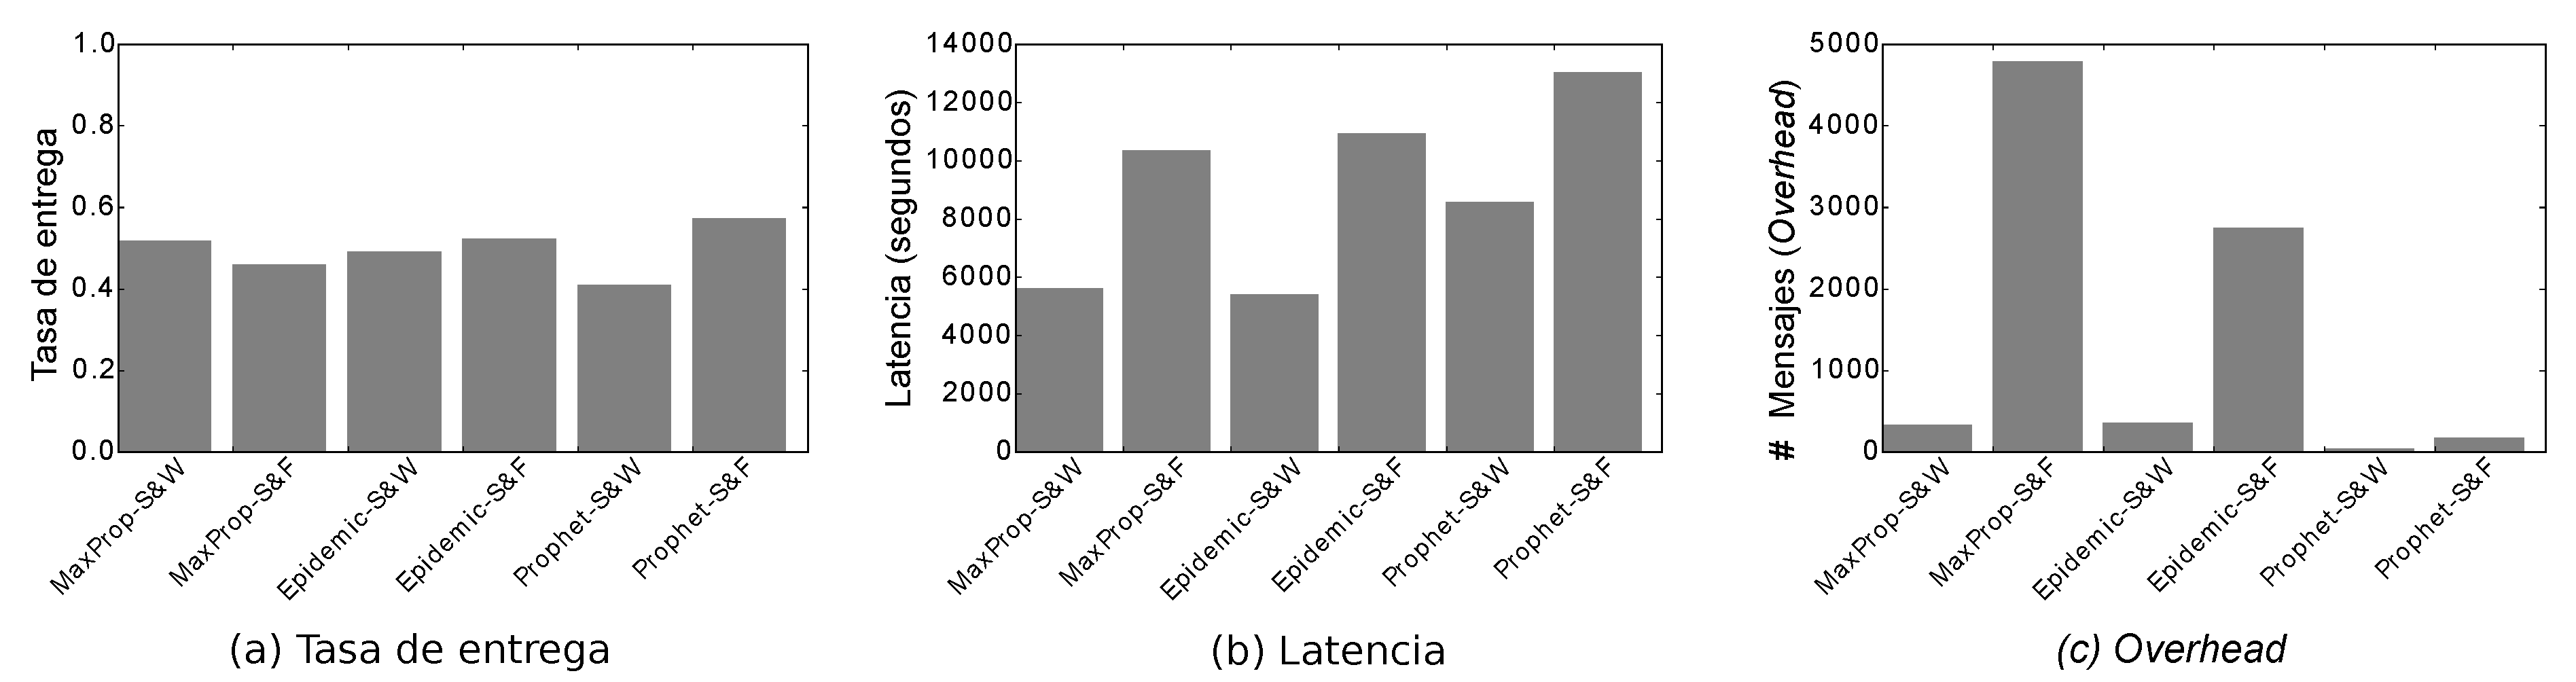
\includegraphics[scale=0.27]{desarrollo/paper_pasado/graficos/entre_centros.eps}}{fig:c-c-meta}
{Elaboración propia, (2015)}


\figuraFuente{Tasa de entrega de mensajes entre todos los nodos, \textit{MetaRouter}.}
{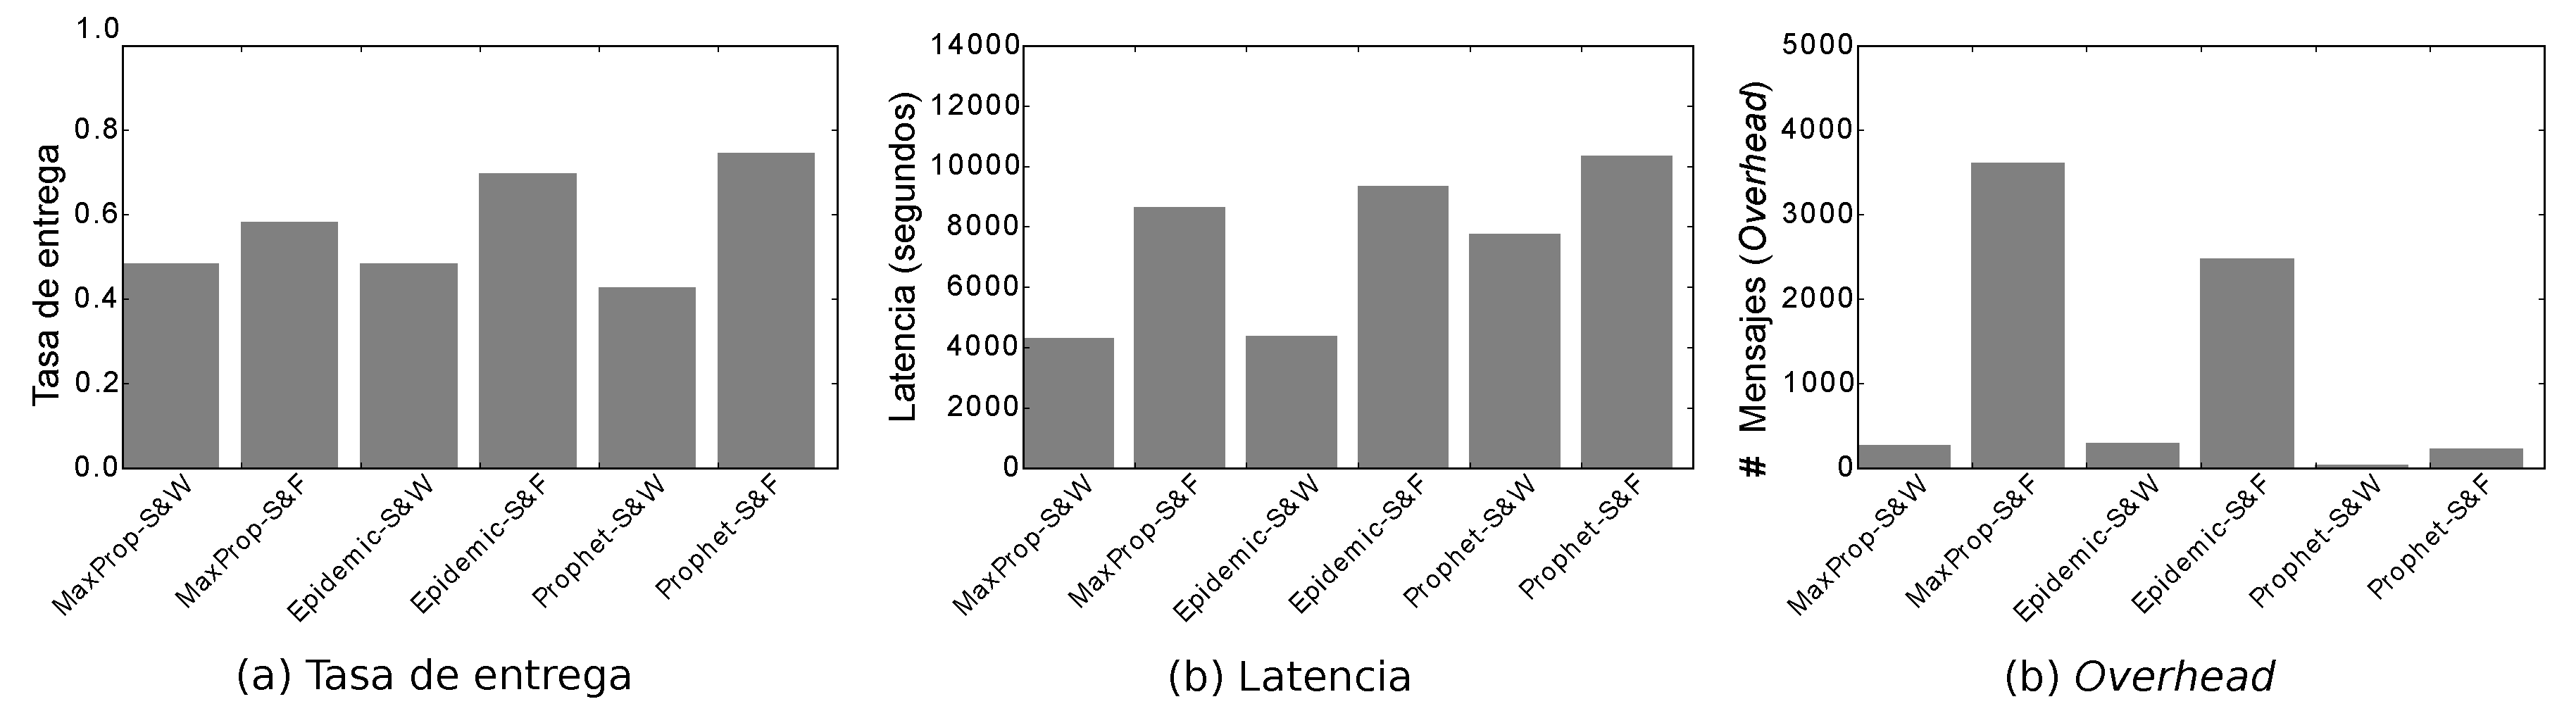
\includegraphics[scale=0.27]{desarrollo/paper_pasado/graficos/todos.eps}}{fig:t-t-meta}
{Elaboración propia, (2015)}


En la \ref{fig:p-c-meta}, \ref{fig:c-c-meta} y \ref{fig:t-t-meta} se pueden ver
los resultados de las simulaciones híbridas. Cada barra indica el protocolo
utilizado en el \textit{carrier} y en el \textit{cluster}
(\textit{CARRIER-CLUSTER}). En términos generales estos resultados muestran que
los protocolos híbridos permiten obtener resultados más homogéneos en términos
de tasa de entrega en los tres escenarios planteados. Además, hay una menor tasa
de entrega si se compara \textit{MetaRouter} con los protocolos del estado del
arte, pero también un mejor \overhead.

Para el caso de la tasa de entrega, utilizando \epidemic{} en los nodos con alta
movilidad y \syf{} en los nodos con baja movilidad es que se obtiene la mejor
tasa de entrega en los tres escenarios, sin embargo, al costo de ser uno de los
que más energía de transmisión consumo debido al alto \overhead{}.

Considerando el \overhead{} de los protocolos, la mezcla que peor desempeño
tiene es \maxprop{} con \syf{} llegando incluso a ser mayor en el caso de
mensajes entre centros si se compara con los experimentos anteriores,
posiblemente debido a la cantidad de réplicas que se generan con \maxprop{}
dentro de un \textit{cluster} de personas.

Realizando un análisis general, la versión híbrida de \prophet{} tiene una
reducción de \overhead{} de un $92\%$ cuando es utilizado con \syf{} y un $98\%$
menos cuando es utilizado con \syw. Sin embargo, la tasa de entrega se ve
reducida en un $10\%$ comparadas con los resultados del protocolo puro y en un
$27\%$ cuando se compara con la mejor tasa de entrega obtenida por \maxprop. A
pesar de esta reducción de la tasa de entrega, la reducción del consumo de
energía (\overhead) es más del $92\%$ que la de \maxprop.


En términos de latencia, viendo la mezcla con mejor resultado (\prophet-\syf) en
términos de tasa de entrega contra consumo de energía es el que obtiene peor
latencia, es decir, los mensajes se demoran más en llegar a los destinos. Esto
puede hacer que no sea viable para ciertas aplicaciones que requieren que los
mensajes se entreguen de forma rápida, pero es la compensación que se debe hacer
para evitar consumir las baterías de los disposivos.


Para analizar la escalabilidad de \textit{MetaRouter} se hicieron experimentos
que muestran el comportamiento del protocolo ante cambios de nodos y cantidad de
mensajes.


\figuraFuente{\textit{Overhead} de comunicación para mensajes hacia centros (P-C),
centros a centros (C-C) y entre todos los participantes de la red (P-P) usando
\textit{MetaRouter}.}
{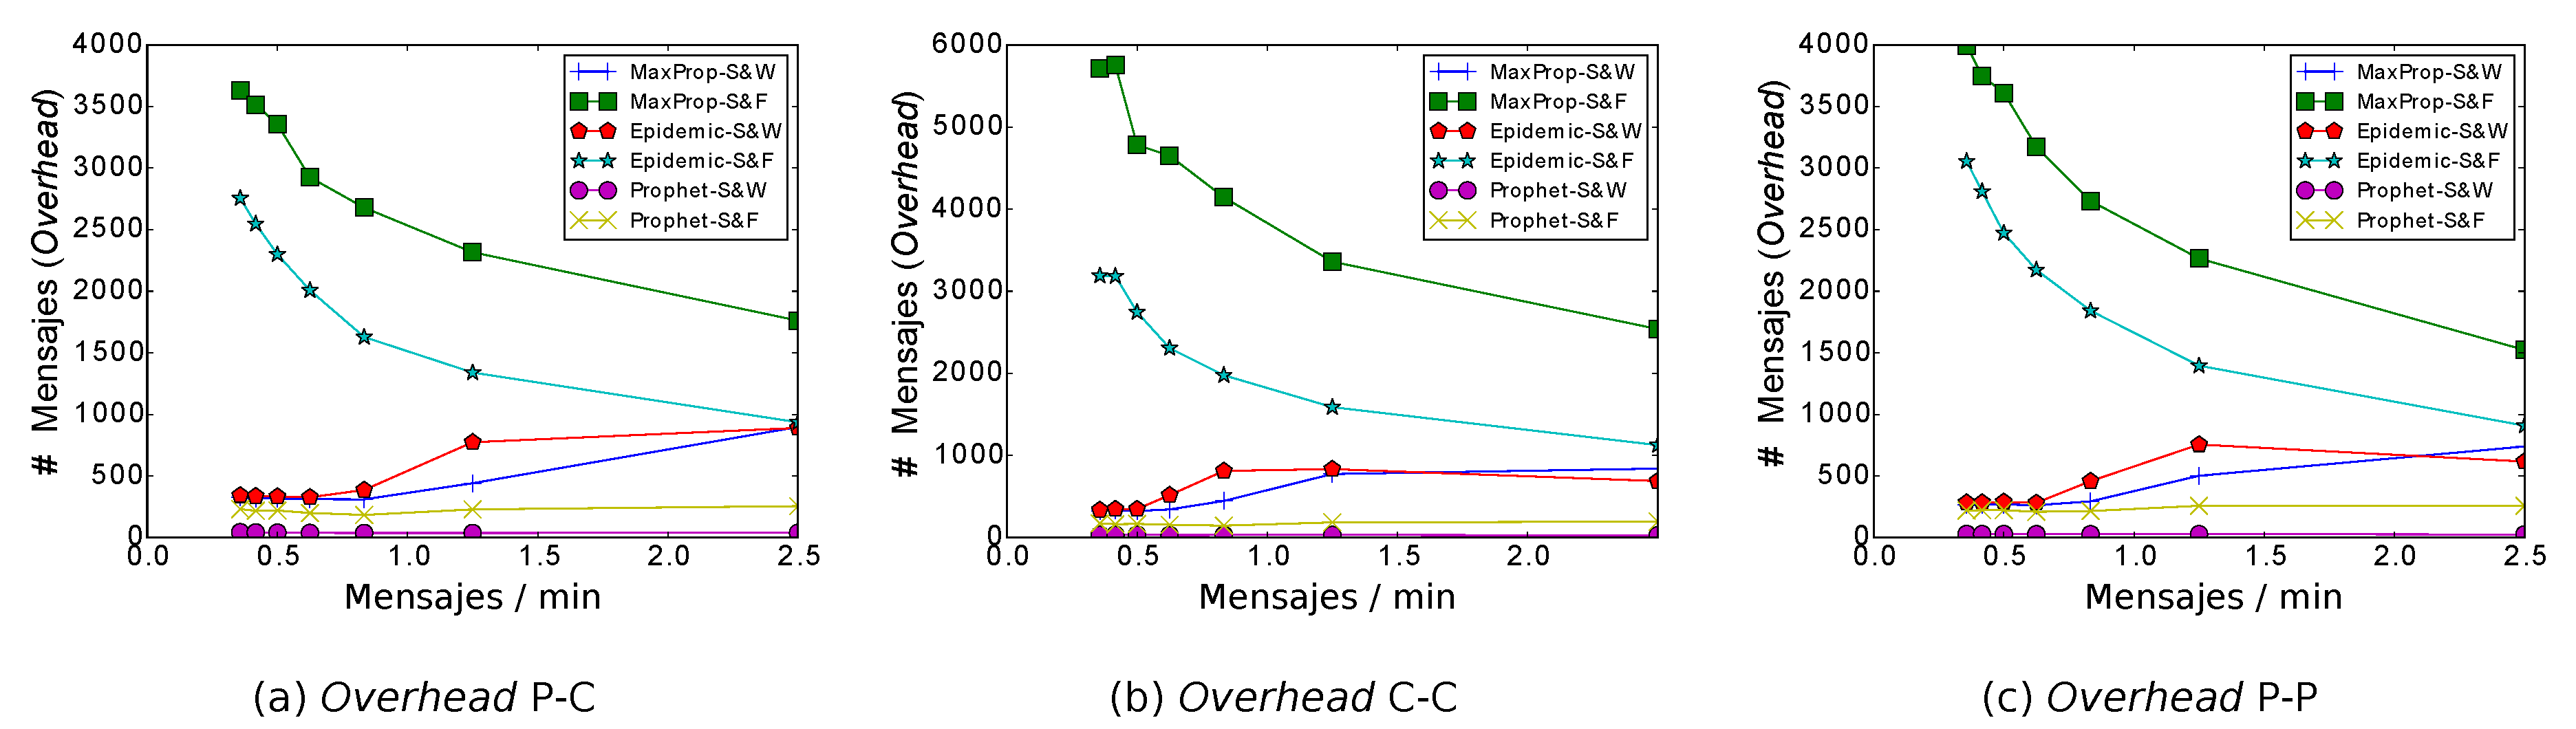
\includegraphics[scale=0.27]{desarrollo/paper_pasado/graficos/lineas/desde_personas_mensajes.eps}}{fig:mensajes-meta}
{Elaboración propia, (2015)}


\figuraFuente{Tasa de entrega para tamaños de mensajes hacia centros (P-C),
centros a centros (C-C) y entre todos los participantes de la red (P-P) usando
\textit{MetaRouter}.}
{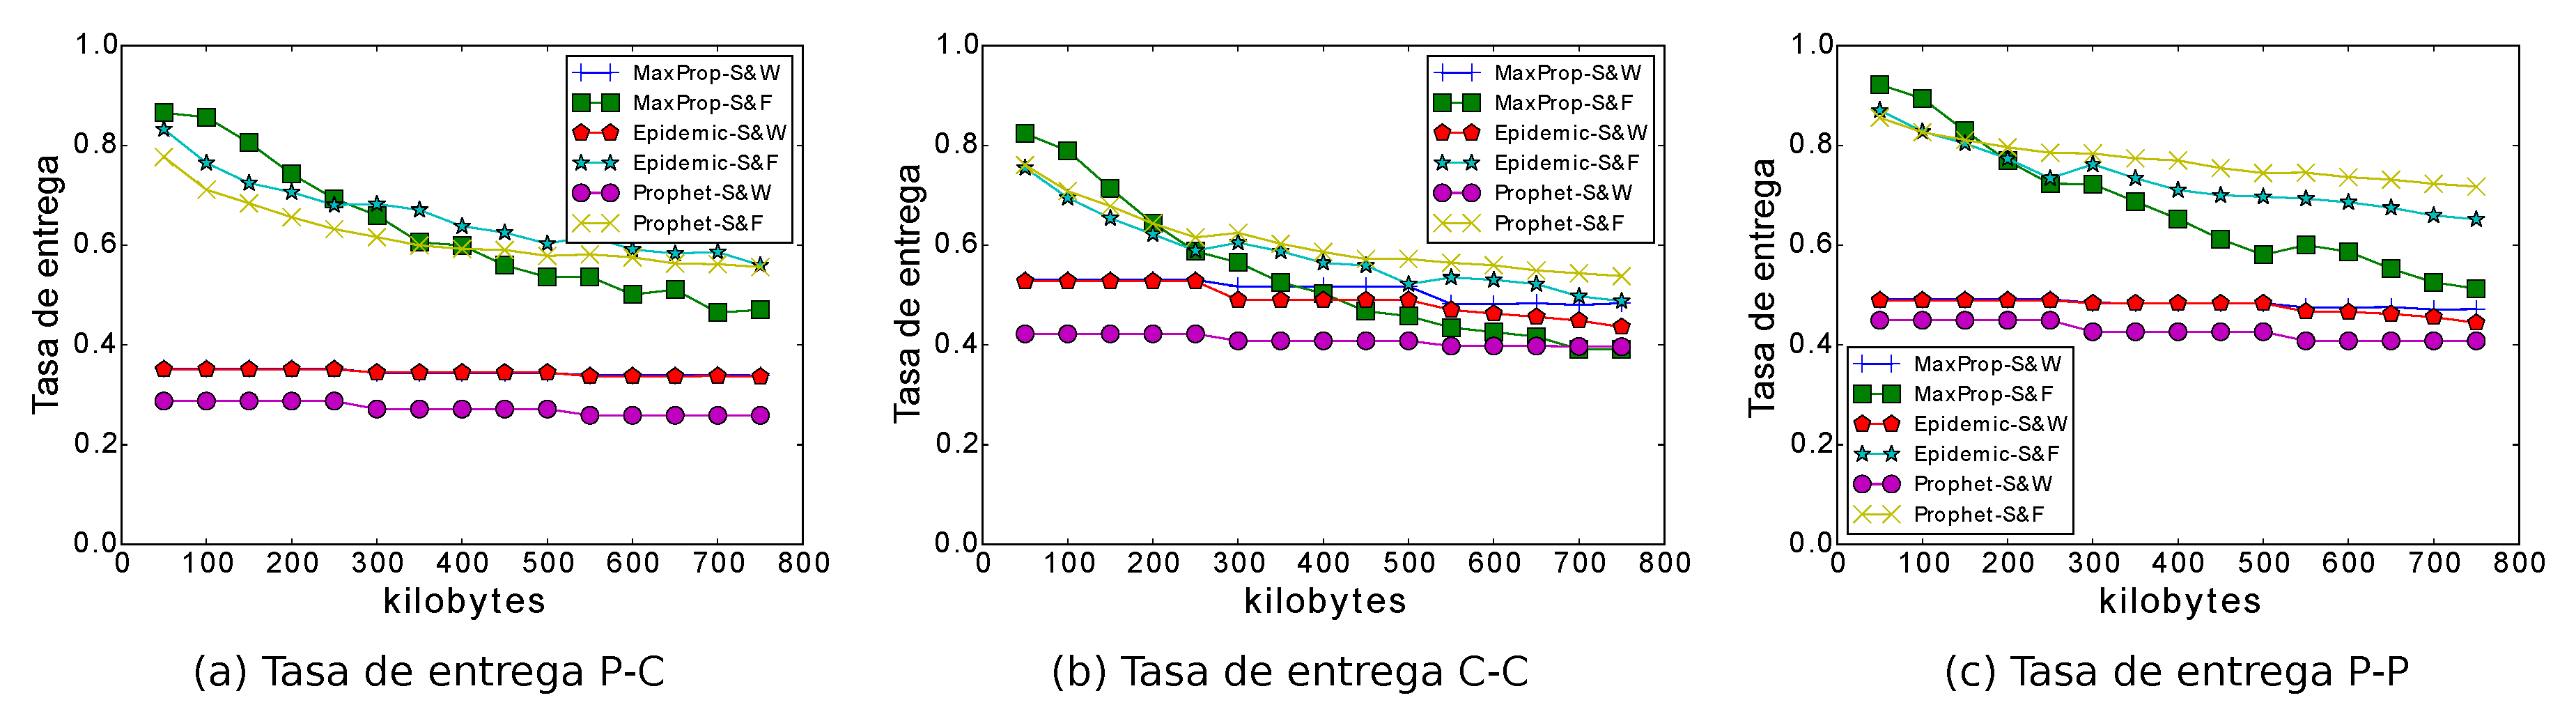
\includegraphics[scale=0.27]{desarrollo/paper_pasado/graficos/lineas/delivery_size.eps}}{fig:size-meta}
{Elaboración propia, (2015)}


\figuraFuente{\textit{Overhead} de comunicación para distintas cantidades de personas en los
\textit{clusters}/vecindarios hacia centros (P-C), centros a centros (C-C) y
entre todos los participantes de la red (P-P) usando \textit{MetaRouter}.}
{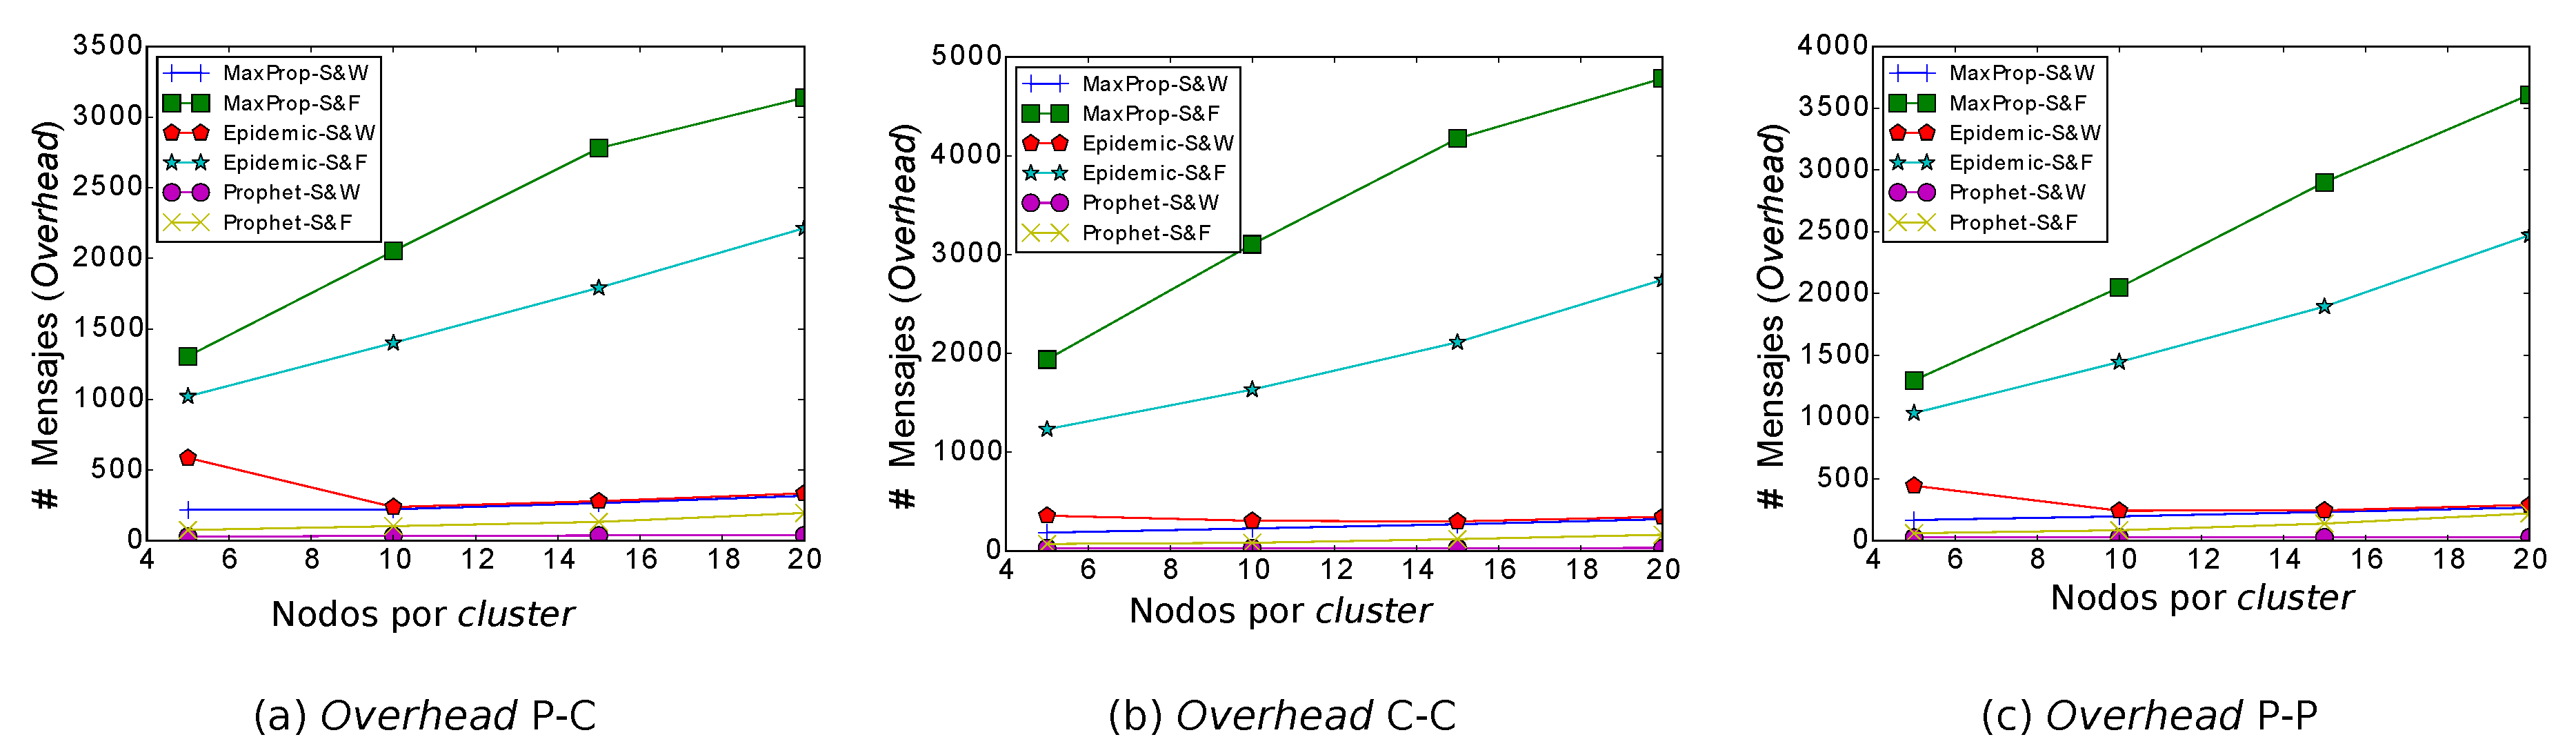
\includegraphics[scale=0.27]{desarrollo/paper_pasado/graficos/lineas/delivery_personas.eps}}{fig:delivery-meta}
{Elaboración propia, (2015)}

Cuando se varía la cantidad de mensajes generados por minuto en la red en la
\ref{fig:mensajes-meta} se encuentra que a mayor saturación de la red, menor es
el \overhead. La explicación de este fenómeno se puede explicar si se sabe que
los \textit{buffers} tienden a quedar libres cuando hay pocos mensajes en la
red, entonces hay menos mensajes descartados para hacer espacio a los que van
llegando al nodo, razón por la cual es posible generar muchas más copias por
mensajes dentro de la red.


En la \ref{fig:size-meta} se analizó el impacto que tiene el tamaño del
mensaje en diferentes protocolos híbridos. Los resultados muestran que el tamaño
de mensaje no afecta protocolos como \prophet-\syw, \maxprop-\syw{} y
\epidemic-\syw, probablemente debido a que su bajo \overhead{} mantiene los
\textit{buffers} sin ocupar su máxima capacidad evitando que sean descartados
los más viejos para hacer espacio a los que van llegando y a que mientras mayor
es el tamaño de mensaje, menos espacio hay para almacenarlos.  Por otro lado,
los protocolos mezclados con \syf{} degradan su desempeño cuando aumenta el
tamaño del mensaje causado por el mismo problema de mantener mensajes en el
\textit{buffer} dado que este último protocolo requiere que los mensajes se
encuentren almacenados más tiempo para llegar a su destino.

Finalmente, la \ref{fig:delivery-meta} muestra lo que sucede cuando se varía la
cantidad de nodos por vecindario en la simulación para analizar como varía el
desempeño de la red respecto al consumo de energía. Mientras más nodos hay en la
red, mayor es el consumo de energía de las mezclas con \syf{} debido a las
razones dadas anteriormente: más personas significa que hay más \textit{buffers}
disponibles en la red y por lo tanto mayor posibilidad de generar copias. El
resto de los protocolos se comporta de manera lineal.


Estos resultados indican que se puede hacer una relación entre el \overhead{}
generado por un protocolo y como se va a ver afectada esta métrica. Un mayor
\overhead{} implica que cuando se escala la red a una mayor cantidad de nodos o
mayor cantidad de mensajes, tiende a explotar la cantidad de copias de mensajes
en la red que se traduce en un mayor consumo de energía. Por otro lado,
protocolos que tienen un bajo \overhead{} tienen a tener un desempeño lineal para
las variables utilizadas.



\seccion{Conclusiones del protocolo estático}

En este capítulo se presenta la motivación, diseño, implementación y pruebas de
\textit{MetaRouter}, un protocolo estático para crear redes DTN híbridas. Se
demuestra que escenarios de desastres donde la energía es escasa pueden verse
beneficiados de este tipo de redes al aplicar un conjunto de reglas de
enrutamiento (protocolo) a cada nodo dependiendo de su patrón de movilidad para
mejorar el consumo de energía mediante una compensación entre tasa de entrega y
\overhead{} de mensajes, siendo este último causa directa del consumo de energía
de transmisión comprobando la hipótesis al principio del capítulo.


En general se puede decir que protocolos híbridos entregan una buena compensación
entre tasa de entrega y \overhead{} de mensajes. En el escenario de desastre
basado en el modelo de movilidad PDM, los mejores resultados se obtuvieron al
combinar \prophet{} con \syf. La importante reducción del \overhead{} generado
permite un mejor uso de la energía por parte de los dispositivos que participan
en la red permitiéndole a esta sobrevivir mayor tiempo.

En los siguientes capítulos se va a presentar el diseño de un nuevo protocolo
híbrido utilizando como base lo que se aprendió con \textit{MetaRouter}. Este
nuevo protocolo va a cambiar la asignación estática por una dinámica basada en
contextos.
